\part{Concept}%

\chapter{Interaction of Light and Matter}
Traditionally cells have been studied with optical light. To
understand why light is a good probe to study cells, it is necessary
to understand the nature of its interaction with matter. For most work
described in this thesis the classical model \DIFaddbegin \DIFadd{of }\DIFaddend describing light as a
wave \DIFdelbegin \DIFdel{is sufficient. This chapter }\DIFdelend \DIFaddbegin \DIFadd{works well. In this chapter we }\DIFaddend will create the mathematical
framework that describes \DIFaddbegin \DIFadd{how light behaves in }\DIFaddend our diffraction
experiments.

\section{Light as electromagnetic radiation}
In the 17th and 18th century it became possible for humans to generate
\DIFdelbegin \DIFdel{continuous }\DIFdelend electric charges and \DIFaddbegin \DIFadd{continuous }\DIFaddend currents [Guericke, Leiden, Volta],
enabling the investigation of the phenomena of electricity and
magnetism. This ultimately led to \DIFdelbegin \DIFdel{the ground breaking work of Maxwell
. His four laws are the synthesis of the }\DIFdelend \DIFaddbegin \DIFadd{a ground-breaking work by Maxwell
where he ties together the }\DIFaddend fields of magnetism, electricity, and
\DIFaddbegin \DIFadd{somewhat }\DIFaddend surprisingly, optics. \DIFaddbegin \DIFadd{His resutls are described by four
equations known as the Maxwell equations:

}\DIFaddend 

\begin{equation} \nabla \cdot   \vec{E} = \frac{\rho}{\varepsilon_0 }\label{eq:maxlaw1}\end{equation}
\begin{equation} \nabla \cdot   \vec{B} = 0 \label{eq:maxlaw2}\end{equation}
\begin{equation} \nabla \times \vec{E} = -\frac{d\vec{B}}{dt}\label{eq:maxlaw3}\end{equation}
\begin{equation} \nabla \times \vec{B} = \mu \DIFdelbegin \DIFdel{_0 }\DIFdelend \vec{J} -\mu\varepsilon\frac{d\vec{E}}{dt}\label{eq:maxlaw4}\end{equation}

\DIFaddbegin \DIFadd{Here, }\DIFaddend $\vec{E}$ is the electric field, $\vec{B}$ is the magnetic
field, $\varepsilon$ \DIFdelbegin \DIFdel{is the permittivity of a material, and }\DIFdelend \DIFaddbegin \DIFadd{and }\DIFaddend $\mu$ is \DIFdelbegin \DIFdel{its
permeability}\DIFdelend \DIFaddbegin \DIFadd{respectively the permittivity and
permeability of the material}\DIFaddend . \DIFaddbegin \DIFadd{$\rho$ is the charge density and
$\vec{J}$ describes the local current.
}\DIFaddend %Equation \ref{eq:maxlaw1} shows that the electric flux
%leaving a volume is proportional to the charge inside. Equation
%\ref{eq:maxlaw2} states that the magnetic flux leaving a volume is
%always 0. This means that the north and south pole of a magnet are
%always connected, which finds its origin in the dipole moment of the
%electron itself. Equation \ref{eq:maxlaw3} shows that the voltage
%induced in a closed loop in proportional to the rate of change of the
%magnetic flux that the loop encloses. A dynamo uses this phenomena to
%generate a charge. Equation \ref{eq:maxlaw4} shows that the magnetic
%field induced around a closed loop is proportional to the electric
%current plus the rate of change in the electric field. Electric motors
%exploit this phenomena. 
\DIFdelbegin \DIFdel{The main concept lying within these laws }\DIFdelend \DIFaddbegin \DIFadd{An important consequence of these equations }\DIFaddend is that a moving electric
charge will induce a magnetic field, which in \DIFdelbegin \DIFdel{its turn induces }\DIFdelend \DIFaddbegin \DIFadd{turn will induce }\DIFaddend a
change in the electric field, and so on.

In order to understand why these laws unify magnetism, electricity and
optics, we \DIFdelbegin \DIFdel{have to }\DIFdelend \DIFaddbegin \DIFadd{will }\DIFaddend consider a special case: vacuum. In vacuum there are
no localized charges ($\rho = 0$) and no currents ($\vec{J}=0$), which
simplifies equation \ref{eq:maxlaw1} and \ref{eq:maxlaw4} \DIFdelbegin \DIFdel{. 
}\DIFdelend \DIFaddbegin \DIFadd{to

}\DIFaddend 

\begin{equation} \nabla \cdot   \vec{E} = 0 \label{eq:maxlaw1_vac}\end{equation}
\begin{equation} \nabla \times \vec{B} = -\mu_0\varepsilon_0\frac{d\vec{E}}{dt}\label{eq:maxlaw4_vac}\end{equation}

Furthermore, experiments showed \DIFdelbegin \DIFdel{$\varepsilon = \varepsilon_0 = 8.854\cdot10^{-12} Fm^{-1}$,
and $\mu = \mu_0 = 1.257 \cdot 10^{-7} N A^{-2}$}\DIFdelend \DIFaddbegin \DIFadd{that the permitivity for vacuum,
$\varepsilon_0 = 8.854\cdot10^{-12} Fm^{-1}$, and the permeability for
vacuum $\mu_0 = 1.257 \cdot 10^{-7} N A^{-2}$}\DIFaddend . If we now ask ourselves
what \DIFaddbegin \DIFadd{the }\DIFaddend field change caused by a change in the electric field \DIFdelbegin \DIFdel{(}\DIFdelend \DIFaddbegin \DIFadd{is by
studying the equation }\DIFaddend $\nabla \times( \nabla \times \vec{E}) $ \DIFdelbegin \DIFdel{) }\DIFdelend we can
derive something quite amazing:
\[ \nabla \times( \nabla \times \vec{E}) \DIFdelbegin %DIFDELCMD < { \isdef}%%%
\DIFdelend \DIFaddbegin \DIFadd{= }\DIFaddend \nabla (\nabla \cdot
\vec{E}) -\nabla^2 \vec{E} =-\nabla^2 \vec{E} \] The first equality is
\DIFdelbegin \DIFdel{mathematical}\DIFdelend \DIFaddbegin \DIFadd{a well known mathematical relation}\DIFaddend , and for the second \DIFaddbegin \DIFadd{equality
}\DIFaddend equation \ref{eq:maxlaw1_vac} is used. \DIFdelbegin \DIFdel{Another way of writing this equation
is:
}\DIFdelend \DIFaddbegin \DIFadd{Now let's rewrite the equation
in a different way:
}\DIFaddend \[\nabla \times( \nabla \times \vec{E})=
\nabla\times(-\frac{d\vec{B}}{dt}) \DIFdelbegin %DIFDELCMD < \isdef
%DIFDELCMD < %%%
\DIFdelend \DIFaddbegin \DIFadd{=
}\DIFaddend -\frac{d}{dt}(\nabla\times\vec{B})=\frac{d}{dt}(\mu_0\varepsilon_0\frac{d\vec{E}}{dt})
= \mu_0\varepsilon_0\frac{d^2\vec{E}}{dt^2}\] In the first equality we
used equation \ref{eq:maxlaw3}. In the second equality we used a
general algebraic property. In the third equality we used
\ref{eq:maxlaw4_vac}, and in the last equality we combined the two
time derivatives. Together these equations state that:

\begin{equation}\label{eq:wave_eq}
\frac{d^2\vec{E}}{dt^2} = \frac{1}{\mu_0\varepsilon_0}\nabla^2 \vec{E} = v^2 \nabla^2 \vec{E},      v = \frac{1}{\sqrt{\mu_0\varepsilon_0}}
\end{equation}

Equation \ref{eq:wave_eq} is known as the wave equation, which is used
to describe the propagation of a wave \DIFaddbegin \DIFadd{with the speed $v$}\DIFaddend . Combining
this results with the experimentally determined value for $\mu_0$ and
$\varepsilon_0$ shows that electromagnetic \DIFaddbegin \DIFadd{(EM) }\DIFaddend waves travel at \(3\cdot
10^8 \frac{m}{s}\), which agreed with the \DIFdelbegin \DIFdel{then known }\DIFdelend \DIFaddbegin \DIFadd{value of }\DIFaddend speed of light
\cite{Froome1971} \DIFaddbegin \DIFadd{which was already known at the time of Maxwell}\DIFaddend . This
result strongly hints at the possibility that light \DIFdelbegin \DIFdel{can be }\DIFdelend \DIFaddbegin \DIFadd{is }\DIFaddend an
electromagnetic wave. Further experiments succeeded in demonstrating
the existence of \DIFdelbegin \DIFdel{long-wavelength electromagnetic waves }\DIFdelend \DIFaddbegin \DIFadd{electromagnetic waves with long wavelengths }\DIFaddend and
showed that their properties are consistent with the properties of
visible light, including their velocity. Visible light has now become
part of the broader spectrum of electromagnetic radiation. Although
Quantum Mechanics \DIFdelbegin \DIFdel{turned }\DIFdelend \DIFaddbegin \DIFadd{complicates }\DIFaddend the description of light \DIFdelbegin \DIFdel{as wave upside down}\DIFdelend \DIFaddbegin \DIFadd{further}\DIFaddend , many
phenomena can be described by treating light as a \DIFaddbegin \DIFadd{pure }\DIFaddend wave.

\section{Photon-material interactions}
Assuming that light is electromagnetic radiation, it is easy to
understand that a change in \DIFdelbegin \DIFdel{electric field }\DIFdelend \DIFaddbegin \DIFadd{the electric field itself }\DIFaddend will affect its
propagation. There are four mechanisms through which radiation
interacts with matter: photo-absorption, scattering, photo-nuclear
absorption and pair production. The latter two phenomena only occur
when matter is exposed to high energy gamma rays, and are therefore of
little relevance to this thesis. \DIFdelbegin \DIFdel{Photo-absorption }\DIFdelend \DIFaddbegin \DIFadd{Photoabsorption }\DIFaddend is facilitated
primarily through \DIFdelbegin \DIFdel{the process of photo-excitation/photo-ionisation of electrons}\DIFdelend \DIFaddbegin \DIFadd{a process called photoexcitation, in which an
electron is excited to a higher level of energy, or possibly ionized
in case of photoionisation }\footnote{\DIFadd{Photoionisation is the process
  that underlies the photo-electric effect.}}\DIFaddend . Scattering can be
divided into two classes: elastic scattering and inelastic
scattering. \DIFdelbegin \DIFdel{In a scattering process the direction of the radiation is changed. }\DIFdelend Elastic scattering does not result in a change of kinetic
energy of the scattering particle, nor does it change the wavelength
of the radiation. \DIFaddbegin \DIFadd{Only the direction of the radiation can be
changed. }\DIFaddend Inelastic scattering leads to both a change in wavelength of
the radiation, and a change in kinetic energy\DIFdelbegin \DIFdel{of the scatterer}\DIFdelend . Photo-absorption and
inelastic scattering deposit energy into the object which will lead to
structural changes \DIFdelbegin \DIFdel{. }\DIFdelend \DIFaddbegin \DIFadd{of the object. These phenomena are therefore not
very useful to study objects structurally. }\DIFaddend Elastic scattering on the
other hand can be used to gain structural information about the
object, without \DIFdelbegin \DIFdel{altering the structure}\DIFdelend \DIFaddbegin \DIFadd{causing damage to the object}\DIFaddend .

\DIFdelbegin \subsection{\DIFdel{Scattering by a single free electron}}
%DIFAUXCMD
\addtocounter{subsection}{-1}%DIFAUXCMD
\DIFdelend \DIFaddbegin \section{\DIFadd{Diffraction}}
\DIFaddend The simplest example of elastic scattering is Thompson scattering from
a free electron. A free electron will scatter \DIFdelbegin \DIFdel{(or diffract ) }\DIFdelend \DIFaddbegin \DIFadd{or diffract }\DIFaddend the incoming
radiation in all directions. \DIFaddbegin \DIFadd{If more than one electron are present
interestingly the scattered waves from the different electrons will
interfere, similar to the interference of water waves. The resulting
pattern of dark and light bands is called a diffraction pattern. The
first person to report this phenomenon was Grimaldi in 1660. Whether
the interference is constructive or destructive depends on the optical
path difference (OPD) between the scattered waves. Figure
\ref{fig:scatwave} is a schematic of such scattering. Waves with path
differences close to integer number of wavelengths interfere
constructively, if close to half integer number of wavelengths the
waves will interfere destructively. The central light band is often
referred to as the zeroth diffraction order, or more colloquially as
the central speckle. The light band next to it is called the first
diffraction order, the one next to that the second order and so on.

}

\subsection{\DIFadd{Lorentz Force}}\label{sec:thom_scat}
\DIFaddend An important physical concept for understanding scattering on a deeper
level is the Lorentz force \DIFdelbegin \DIFdel{. 
}\DIFdelend \DIFaddbegin \DIFadd{which describes the force exerted on a
charged particle traveling in an electromagnetic field:
}\DIFaddend \begin{equation}\label{eq:lorentz}
\vec{F} = q\vec{E} + q\vec{v}\times\vec{B}
\end{equation} 

\DIFaddbegin \DIFadd{Here $\vec{v}$ describes the speed and direction of movement of the
particle and $q$ its charge. }\DIFaddend From Newton's second law of motion
($\vec{F} = m \vec{a}$) it is known that force and acceleration are
proportional and parallel, thus the Lorentz force describes the
acceleration of a charge in an electric and/or magnetic field. The
first term of equation \ref{eq:lorentz} is also known as the Coulombic
force, and shows that a charge is accelerated in the direction of an
electric field. The second term shows that a moving charge is
accelerated by the presence of a magnetic field in the direction that
is both perpendicular to its movement and the magnetic field, given
\DIFaddbegin \DIFadd{that }\DIFaddend $\vec{v}$ and $\vec{B}$ are not parallel \DIFdelbegin \DIFdel{(in that }\DIFdelend \DIFaddbegin \DIFadd{in which }\DIFaddend case there is
no acceleration\DIFdelbegin \DIFdel{)}\DIFdelend .

\DIFaddbegin \subsection{\DIFadd{Scattering by a single free electron}}
\DIFaddend According to classical electromagnetic theory the electric field
associated \DIFdelbegin \DIFdel{to }\DIFdelend \DIFaddbegin \DIFadd{with }\DIFaddend a monochromatic plane wave of \DIFdelbegin \DIFdel{strength }\DIFdelend \DIFaddbegin \DIFadd{amplitude }\DIFaddend $E_0$ \DIFdelbegin \DIFdel{, }\DIFdelend \DIFaddbegin \DIFadd{and
}\DIFaddend wavelength $\lambda$, propagating in the z-direction \DIFdelbegin \DIFdel{(longitudinal direction) }\DIFdelend can be described
by:

\begin{equation}\label{eq:plane_wave}
\vec{E_{in}} = E_0 e^{-2\,\pi\ i \frac{ c t }{\lambda}}
\end{equation} 

When the oscillating electric field of the incident EM wave hits a
stationary electron of mass $m_e$ and charge $e$ \DIFdelbegin \DIFdel{(}\DIFdelend located at
position $z = 0$\DIFdelbegin \DIFdel{)}\DIFdelend , it exerts a Coulombic force on the electron which
causes it to oscillate at the same frequency as the incident
radiation. By Newton's second law of motion:

\begin{equation}\label{eq:motion_single}
\vec{F} = m_e \vec{a} = e E_0 e^{-2\,\pi\ i \frac{ c t}{\lambda}} 
\end{equation}

An accelerated charge emits electromagnetic radiation, since this is
the only mechanism through which the electron can preserve
momentum. The oscillating electron becomes a new source of radiation
that radiates spherically in all directions, at the same frequency as
the incident radiation. This phenomenon is called Thompson
scattering. From Maxwell's equations it follows that the electric
field generated by an accelerating electron measured at point
$\vec{d}$ can be described as:

\begin{equation}\label{eq:scattering}
\vec{E_s}(\vec{d},t) = \DIFdelbegin \DIFdel{\frac{e a_\perp(t-|\vec{d}|/c)}{4 \pi \varepsilon_0c^2d}
}\DIFdelend \DIFaddbegin \DIFadd{\frac{e a_\perp(t-|\vec{d}|/c)}{4 \pi \varepsilon_0c^2|\vec{d}|}
}\DIFaddend \end{equation}

$a_{\perp}$ is the acceleration projected on a plane perpendical to
$\vec{d}$. Combining equations \ref{eq:plane_wave},
\ref{eq:motion_single} \DIFdelbegin \DIFdel{, }\DIFdelend \DIFaddbegin \DIFadd{and }\DIFaddend \ref{eq:scattering} we get that the
instantaneous scattered field is:
\begin{align*}
a_\perp =& |\vec{a(t)}|\sin(\theta)\\
E_s(\vec{d},t) =& \frac{{e}^2}{4 \pi \varepsilon_0 m_e\,c^2} \frac{E_0 \sin(\theta)}{d} e^{-2\,\pi\ i \frac{|\vec{d}|}{\lambda}}
\end{align*}

The classical electron radius $r_e$ can be used to simplify the
equation for the scattered field $E_s$
\begin{align*}
E_s=& - \frac{r_e\,E_0\,\sin(\theta)}{d} e^{-2\,\pi\ i \frac{|\vec{d}|}{\lambda}}\\
r_e =& \frac{e^2}{4 \pi \varepsilon_0 m_e\,c^2}    
\end{align*}


\subsection{\DIFdelbegin \DIFdel{Two-body scattering}\DIFdelend \DIFaddbegin \DIFadd{Scattering from two electrons}\DIFaddend }
%\subsection{Approximations} 

\DIFdelbegin \DIFdel{If more than one electron are presentthe scattered waves will interfere, similar to the interference of water waves. The resulting pattern of dark and light bands is called a diffraction pattern. The first person to report this phenomenon was Grimaldi in 1660. Whether the
interference is constructive of destructive depends on the optical path difference (OPD) between the scattered waves. Waves with path differences close to integer numbers of wavelengths interfere constructively, if close to half integral waves will interferedestructively. The central light band is often referred to as the zeroth diffraction order, or more colloquially as the central speckle. The light band next to it is called the first diffraction order (or first fringe), the one next to that the second order and so on. These terms will be used throughout the thesis. }\DIFdelend \DIFaddbegin 

\DIFadd{If two electrons are present, instead of one single electron, the
scattered EM waves from both electrons will interfere. }\DIFaddend Figure
\ref{fig:Interference} illustrates \DIFdelbegin \DIFdel{the phenomenonof interference}\DIFdelend \DIFaddbegin \DIFadd{this phenomenon}\DIFaddend .

\begin{figure}[h]\label{fig:Interference}
\centering 
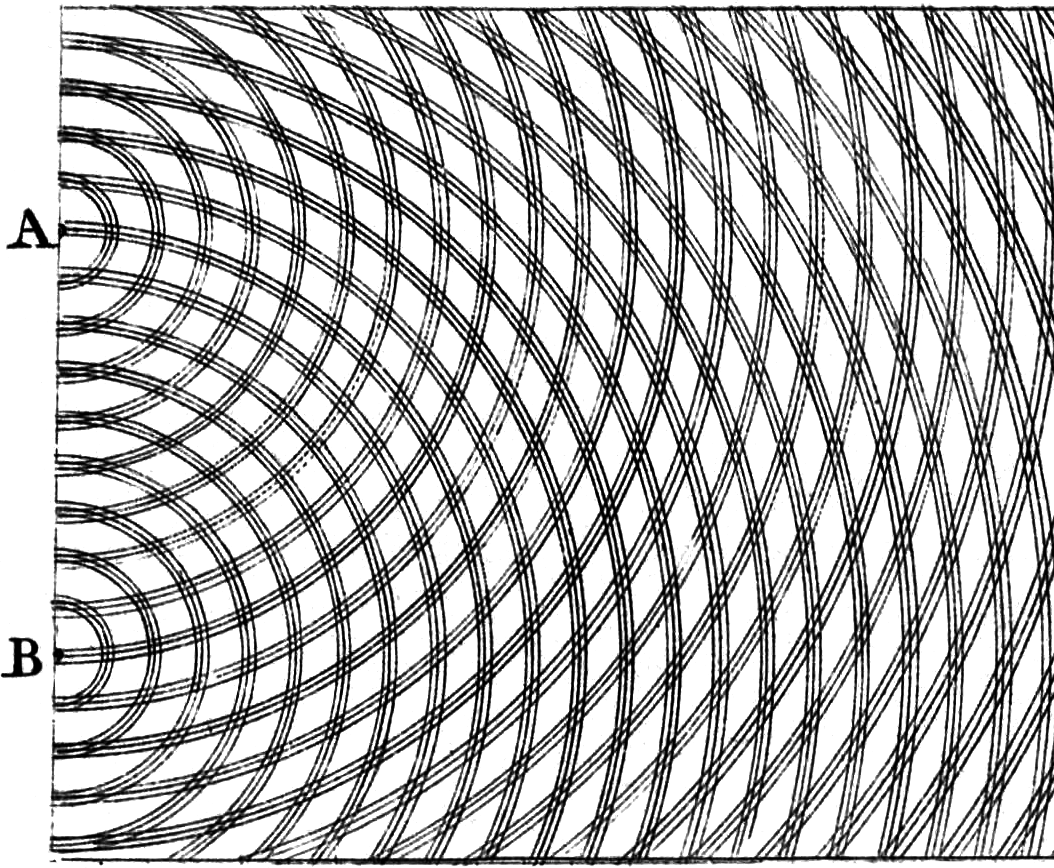
\includegraphics[width=46mm]{Young_Diffraction2.png}
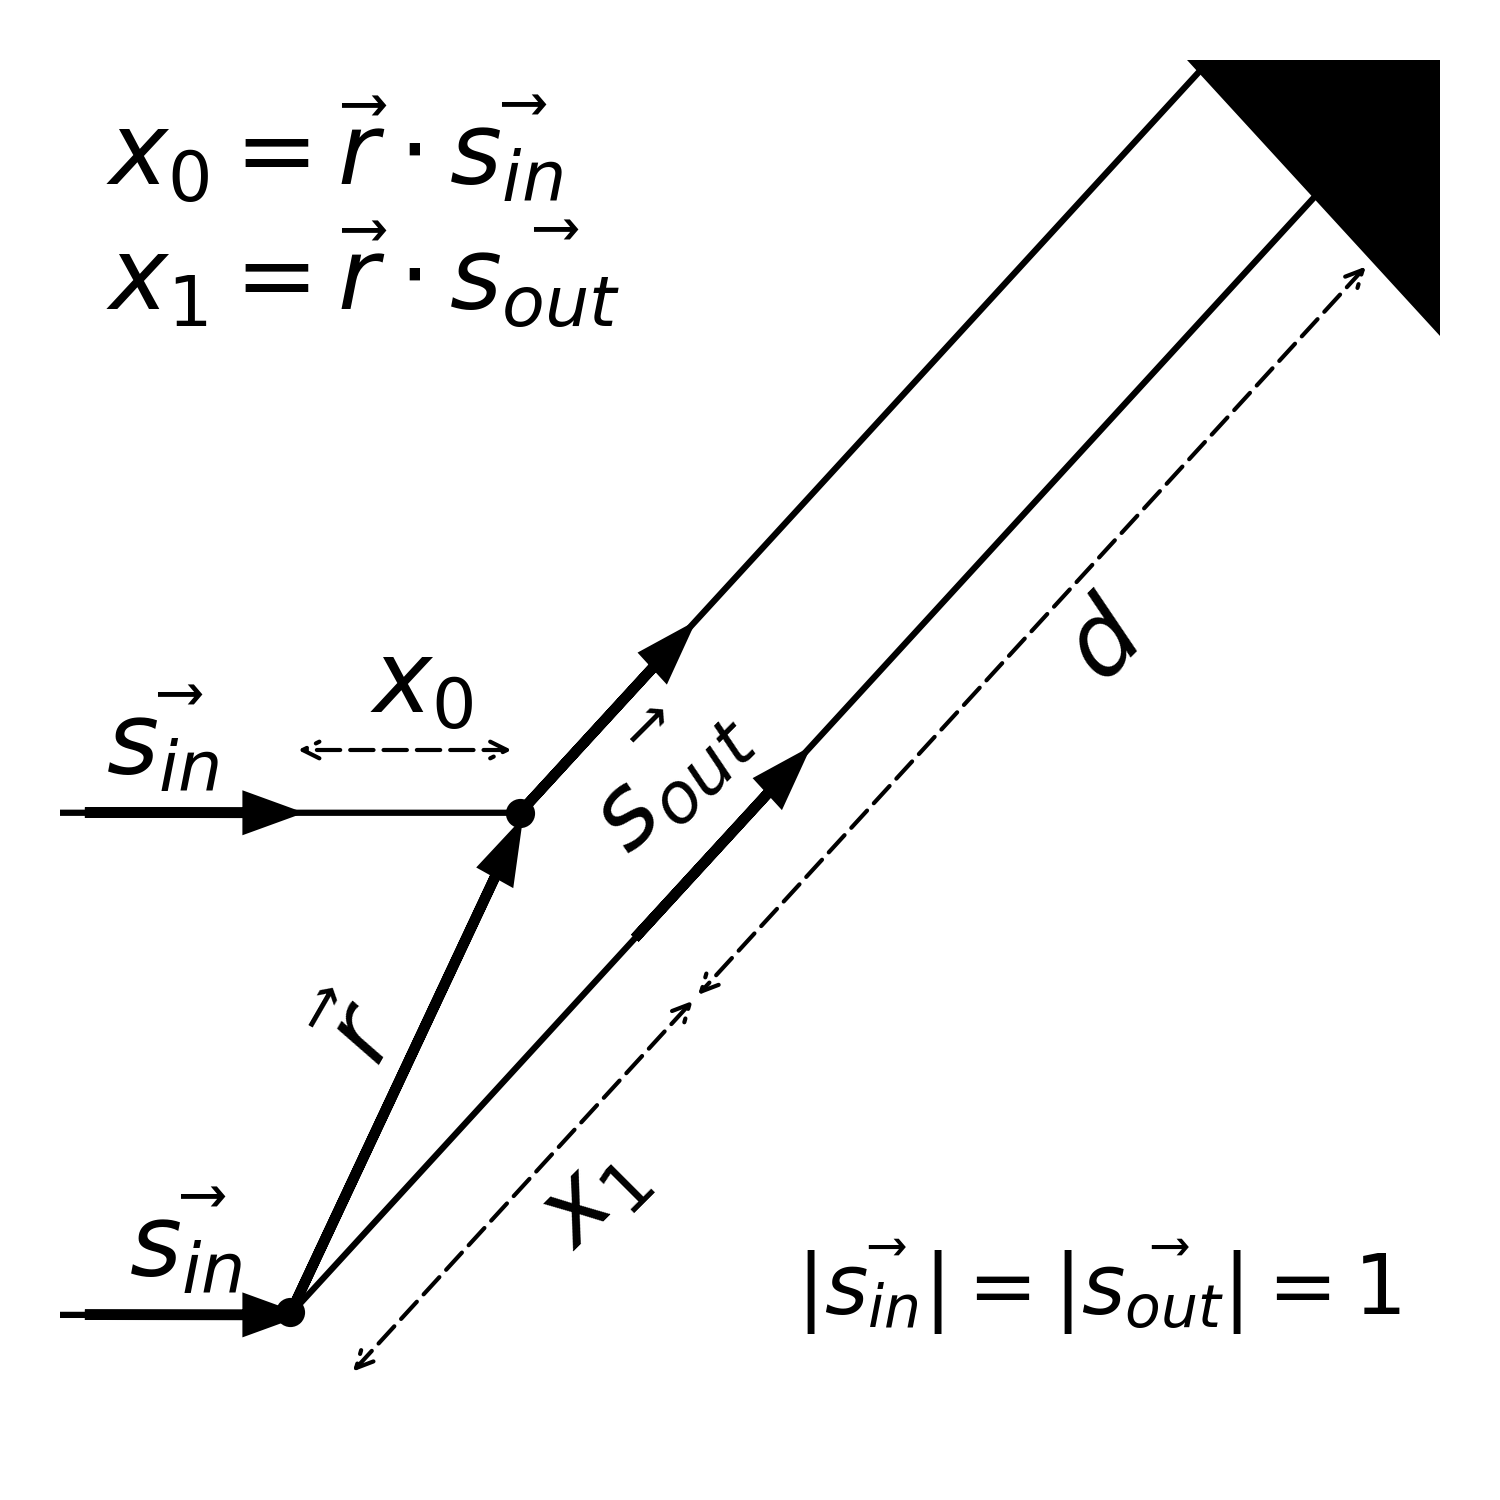
\includegraphics[width=40mm]{blah.png}

\caption{Illustration of scattering from two free-electrons A and
  B. a) graphic taken from Young, showing an interference pattern
  between two waves. b) mathematical description of the path length
  difference \DIFaddbeginFL \DIFaddFL{between }\DIFaddendFL two waves arriving at point
  $\vec{d}$. $\vec{s_{in}}$ and $\vec{s_{out}}$ are unit vectors
  \DIFdelbeginFL \DIFdelFL{point }\DIFdelendFL \DIFaddbeginFL \DIFaddFL{pointing }\DIFaddendFL in the direction of \DIFaddbeginFL \DIFaddFL{propagation of }\DIFaddendFL the incident wave and
  the out going wave \DIFaddbeginFL \DIFaddFL{respectively}\DIFaddendFL . $\vec{r}$ is \DIFdelbeginFL \DIFdelFL{the }\DIFdelendFL \DIFaddbeginFL \DIFaddFL{a }\DIFaddendFL position vector
  \DIFdelbeginFL \DIFdelFL{of }\DIFdelendFL \DIFaddbeginFL \DIFaddFL{describing the distance from }\DIFaddendFL point A \DIFdelbeginFL \DIFdelFL{, compared }\DIFdelendFL to point B. Note that in a)
  $x_0 = 0$.}
\end{figure}

If the diffraction pattern is measured at point \(\vec{d}\), far away
from the diffracting object itself, both scattered fields have
approximately the same field strength \DIFdelbegin \DIFdel{as }\DIFdelend \DIFaddbegin \DIFadd{since }\DIFaddend the distance from both
electrons to the detector is about equal\DIFdelbegin \DIFdel{: }\DIFdelend \DIFaddbegin \DIFadd{. In figure
\ref{fig:Interference} this means that }\DIFaddend $|\vec{d}+x_1| \approx
|\vec{d}|$. This approximation is called the far-field
approximation. The Fresnel number (FN) is used to verify the validity
of the far-field approximation.
\begin{equation} 
FN = \frac{o^2}{d\lambda}
\end{equation}
\DIFaddbegin \DIFadd{where }\DIFaddend $o$ is the object size, $d$ the distance from the object to the
detector, and \(\lambda\) the wavelength of the radiation. The
far-field approximation is valid when $FN \ll 1$. All diffraction
patterns discussed in this thesis are taken in the far-field.

The electric field at point $\vec{d}$ \DIFdelbegin \DIFdel{can be described by a }\DIFdelend \DIFaddbegin \DIFadd{is given by the }\DIFaddend sum of the
\DIFaddbegin \DIFadd{individual }\DIFaddend scattered electric fields:
\begin{equation}
E(\vec{d}) = E_s(\vec{d})+E_s(\vec{d}) e^{\frac{2 \pi\,i\,\Delta x}{\lambda}} 	 
\end{equation}
$\Delta x$ is the optical path difference between \DIFdelbegin \DIFdel{both scattered
}\DIFdelend \DIFaddbegin \DIFadd{the two scattered
waves }\DIFaddend due to the relative difference in position. $\Delta x$ can \DIFdelbegin \DIFdel{also be
}\DIFdelend \DIFaddbegin \DIFadd{be
determined by summing $x_0$ which is the path difference of the
incoming radiation and $x_1$ which is the path difference of the
outgoing radiation.  be }\DIFaddend described using the difference vector r:
\begin{equation}
\Delta x = x_0 - x_1 =\vec{s_{out}} \cdot \vec{r}-\vec{ s_{in}}\cdot \vec{r} = (\vec{s_{out}} -\vec{s_{in}} ) \cdot \vec{r} 
\end{equation}

By defining the scattering vector $\vec{S}$
\begin{equation}
\vec{S} = \frac{\vec{s_{out}}-\vec{s_{in}} }{\lambda}
\end{equation}
the diffraction pattern of two electrons will be 
\DIFdelbegin \DIFdel{:
}\begin{displaymath}
\DIFdel{E(\vec{d}) = E_s(\vec{d}) + E_s(\vec{d}) e^{2\,\pi\,  i\,\vec{S}\cdot\vec{r}}
}\end{displaymath}
%DIFAUXCMD
\DIFdelend \DIFaddbegin \[\DIFadd{E(\vec{d}) = E_s(\vec{d}) + E_s(\vec{d}) e^{2\,\pi\,  i\,\vec{S}\cdot\vec{r}}}\]

\DIFaddend 

\DIFdelbegin \DIFdel{It is important }\DIFdelend \DIFaddbegin \DIFadd{Important }\DIFaddend to note is that $\Delta x $ \DIFdelbegin \DIFdel{is at most }\DIFdelend \DIFaddbegin \DIFadd{can at most be $|\vec{r}|$, }\DIFaddend the
distance between the two electrons\DIFdelbegin \DIFdel{$|\vec{r}|$}\DIFdelend . Abbe demonstrated that in order to
resolve two electrons from each other at least two diffraction orders
must be captured. This usually means the zeroth and the first
order. The first order start where $\Delta x > \lambda/2$. For two
electrons closer than half a wavelength apart this will never be the
case. This sets a physical limit to the possible details one can
resolve using a regular diffraction set-up. One would not be able to
use green light (\DIFdelbegin \DIFdel{$\lambda = 500\,nm$}\DIFdelend \DIFaddbegin \DIFadd{$\lambda = 500 nm$}\DIFaddend ) to image objects smaller than 250
nm. For structural studies of molecules this means that in order to
distinguish single atoms, X-ray radiation \DIFdelbegin \DIFdel{is }\DIFdelend \DIFaddbegin \DIFadd{will be }\DIFaddend required.


\subsection{Scattering from multiple electrons}
In biological particles the incoming EM radiation is scattered by many
electrons. The electric field can be described as the sum of all the
individual scattered fields.
\begin{equation}\label{eq:boehoe}
E(\vec{d}) = E_s(\vec{d}) \sum_{n} e^{2\,\pi\,  i\,\vec{S}\cdot\vec{r_n}}
\end{equation}
\DIFaddbegin \DIFadd{where $n$ identifies the individual electrons.

}\DIFaddend 

If all electrons together are assumed to form a continuous electric
charge density around the many nuclei that constitute the biological
particle, equation \ref{eq:boehoe} can be written as a continuous
function.
\begin{equation}\label{eq:cont}
E(\vec{d}) = E_s(\vec{d})\int \rho(\vec{r},\lambda) \exp^{-2\pi i \,\vec{S} \cdot \vec{r}}\,d\vec{r}
\end{equation}

$\rho(\vec{r},\lambda)$ is named the scattering potential and takes
the scattering strength of each nucleus into consideration.

So far we have implicitly assumed that the scattered field will not be
scattered a second time. This approximation is called the first Born
approximation. We assume this to be valid for all objects smaller than
a few micrometers.

We can now introduce the scattering factor $F(\vec{S})$.
\begin{equation}
F(\vec{S}) = \frac{E(\vec{d})}{E_s(\vec{d})} = F(\frac{\vec{d}}{|d|}
\end{equation}
The structure factor is independent of the distance of the detector,
it only depends on the angle of measurement. Equation \ref{eq:cont}
can be rewritten as:
\begin{equation}\label{eq:diff_equation}
F(\vec{S}) = \int \rho(\vec{r},\lambda) \exp^{-2\pi i \,\vec{S} \cdot \vec{r}}\,d\vec{r}
\end{equation}
This equation shows that a diffraction experiment is simply the 3D
Fourier transform of the electron density evaluated at $\vec{S}$. This
relation is very convenient as there is a large mathematical field
describing the relations of Fourier transformations. A few of these
relations are very useful to this thesis.

The Fourier shift theorem describes the change in the diffraction
pattern upon object translation\DIFdelbegin \DIFdel{(i.
e. shift).
}\DIFdelend \DIFaddbegin \DIFadd{.
}\DIFaddend \begin{equation}
\mathcal{F}(f(x+\delta x))=e^{2\pi i \delta x q} \mathcal{F}(f)
\end{equation}
\DIFdelbegin \DIFdel{The }\DIFdelend \DIFaddbegin \DIFadd{We see that the translation in real space turns into a multiplication
with the }\DIFaddend factor $e^{2 \pi i \delta x q}$ \DIFaddbegin \DIFadd{which }\DIFaddend is called a
'phase-ramp'.

The Convolution theorem states that a multiplication in Fourier space
is a convolution in \DIFdelbegin \DIFdel{object space (real space ) and vice versa.
}\DIFdelend \DIFaddbegin \DIFadd{real space and visa versa.
}\DIFaddend \begin{equation}
f(x) * g(x) = \int f(\tau)g(x-\tau)\,d\tau = \mathcal{F}^{-1} \DIFdelbegin %DIFDELCMD < {%%%
\DIFdelend \DIFaddbegin \left(\DIFaddend \mathcal{F}\DIFaddbegin \left(\DIFaddend f(x)\DIFdelbegin \DIFdel{\times}\DIFdelend \DIFaddbegin \right)\DIFadd{\cdot}\DIFaddend \mathcal{F}\DIFaddbegin \left(\DIFaddend g(x)\DIFdelbegin %DIFDELCMD < }
%DIFDELCMD < %%%
\DIFdelend \DIFaddbegin \right)\right)
\DIFaddend \end{equation}

%DIF > % The Fourier slice theorem states that a 2D diffraction pattern is a
%DIF > % slice through the center of the 3D fourier transform of the object.
%DIF > % It has thus become possible to move between diffraction pattern and
%DIF > % electron density.
The Fourier slice theorem \DIFdelbegin \DIFdel{states that a }\DIFdelend \DIFaddbegin \DIFadd{relates the Fourier transform of a 3D
density with the Fourier transform of a }\DIFaddend 2D \DIFdelbegin \DIFdel{diffraction pattern is a }\DIFdelend \DIFaddbegin \DIFadd{projection image of the
same density. More precisely it says that the transform of the
projection is identical to a 2D }\DIFaddend slice through the \DIFdelbegin \DIFdel{center }\DIFdelend \DIFaddbegin \DIFadd{transform }\DIFaddend of the 3D
\DIFdelbegin \DIFdel{fourier transform of the object.

It has thus become possible to move between diffraction pattern and electron density.
}\DIFdelend \DIFaddbegin \DIFadd{density such that the slice goes through the origin.

}\DIFaddend 


\subsection{Scattering Potential}
An important term in \DIFdelbegin \DIFdel{equation }\DIFdelend \DIFaddbegin \DIFadd{the previous equations }\DIFaddend that needs further
development is the scattering potential
\DIFdelbegin \DIFdel{of a material }\DIFdelend $\rho(\vec{r},\lambda)$. Mathematically $\rho(\vec{r},\lambda)$ can be
formulated as a function of the refractive index $n$ of a material.
\begin{equation}
\rho(\vec{r},\lambda) = \pi s_{in}^2 (( n(\vec{r},\lambda))^2 -1))
\end{equation}
\DIFdelbegin \DIFdel{$s = \frac{1}{\lambda}$
}\DIFdelend %DIF > $s = \frac{1}{\lambda}$

The refractive index is related to the scattering factors of the
individual atoms in the material.
\begin{equation}
n = 1-\frac{r_e}{2\pi} \lambda^{2} \sum_{i} N_i f_i(0)
\end{equation}
where $r_e$ is the classical electron radius, $\lambda$ is the
wavelength, $N_i$ is the number of atoms per unit volume. The complex
scattering factor in the forward direction $f(0)$ can be described by:
\begin{equation}
f(0) = f_1 + i f_2
\end{equation}
The imaginary part is derived from the atomic photoabsorption cross
section and is a measure of absorption [booklet]. The real part is
related to the imaginary part using the Kramers-Kronig dispersion
relation [Kramers]. At high photon energies $f_1$ approaches the
atomic number of the atoms. The exact value of $f_1$ and $f_2$ at
different photon-energies have been determined experimentally [Henke].

Figure \ref{fig:waterwindow} presents the scattering factors of two
elements: carbon and oxygen. The gray energy range from \DIFdelbegin \DIFdel{282-533 }\DIFdelend \DIFaddbegin \DIFadd{282 - 533 }\DIFaddend eV
(4.40 nm - 2.33 nm) is called the water window. In this region, and
especially towards the \DIFdelbegin \DIFdel{end}\DIFdelend \DIFaddbegin \DIFadd{higher energies}\DIFaddend , oxygen atoms\DIFdelbegin \DIFdel{(thus water) }\DIFdelend \DIFaddbegin \DIFadd{, and thus water,
}\DIFaddend are scattering significantly less than carbon atoms\DIFdelbegin \DIFdel{(i. e. organic biomolecules). }\DIFdelend \DIFaddbegin \DIFadd{. }\DIFaddend The water window
\DIFaddbegin \DIFadd{is }\DIFaddend therefore a good candidate for imaging cells, as the contrast
between two of their main constituents, water and biomolecules, is
enhanced.

\begin{figure}[h]\label{fig:waterwindow}
\centering 
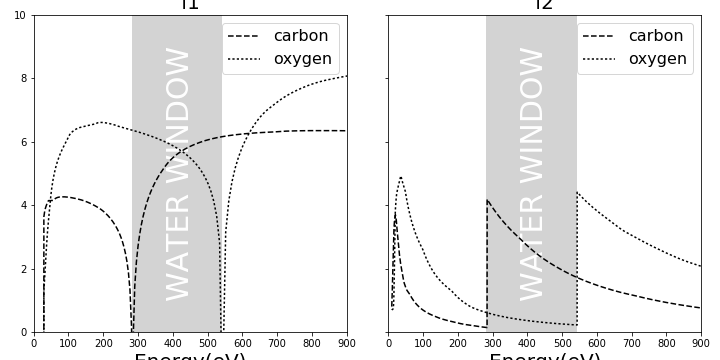
\includegraphics[width=80mm]{waterwindow.png}

\caption{Atomic scattering factors $f_1$ and $f_2$ of carbon and
  oxygen, as a function of photon-energy of the X-ray radiation. The
  region between the absorption K-edge of carbon (282 eV, 4.40 nm) and
  the K-edge of oxygen (533 eV, 2.33 nm) is called the water window.
  The contrast between biomolecules and water is enhanced in this
  region, especially towards the high end of it. These wavelengths
  could be used for imaging living biological particles such as cells
  or organelles.}
\end{figure}

\section{Radiation Damage}
The previous section shows that scattering power of \DIFdelbegin \DIFdel{an }\DIFdelend \DIFaddbegin \DIFadd{a }\DIFaddend body is related
to the wavelength of the radiation. The shorter the wavelength the
less scattering occurs. To compensate for this loss in signal, the
required dose for imaging increases. Practically this means that a
dose in excess of 100 MGy is required to record an interpretable
signal from a living cell\DIFdelbegin \DIFdel{(}\DIFdelend \DIFaddbegin \DIFadd{. This number can be put in perspective by
noting that }\DIFaddend a dose of 2000 Gy is already enough to kill everything
that lives on earth\DIFdelbegin \DIFdel{)}\DIFdelend . Unfortunately other processes of matter-radiation
interaction \DIFaddbegin \DIFadd{also }\DIFaddend become more abundant \DIFdelbegin \DIFdel{as well}\DIFdelend \DIFaddbegin \DIFadd{at lower photon energies}\DIFaddend . At
soft X-ray wavelengths the predominant damage process is
photoionisation. Many \DIFdelbegin \DIFdel{process }\DIFdelend \DIFaddbegin \DIFadd{processes }\DIFaddend follow the ionization, of which
non-radiative Auger decay will lead to significant \DIFdelbegin \DIFdel{radiation }\DIFdelend damage. The
relation between the required dose of radiation versus the maximum
tolerable dose of radiation \DIFdelbegin \DIFdel{posed }\DIFdelend \DIFaddbegin \DIFadd{used to pose }\DIFaddend a physical limit to the obtained
resolution for imaging single biomolecules [Howell].

\section{\DIFdelbegin \DIFdel{Diffract-before-destroy}\DIFdelend \DIFaddbegin \DIFadd{Diffraction before destruction}\DIFaddend }
An elegant solution to the problem of radiation damage \DIFdelbegin \DIFdel{came from the realization that }\DIFdelend \DIFaddbegin \DIFadd{is possible
since }\DIFaddend elastic scattering occurs on a time scale \DIFaddbegin \DIFadd{that is }\DIFaddend shorter than
the \DIFdelbegin \DIFdel{damage processes manifest themselves }\DIFdelend \DIFaddbegin \DIFadd{time it takes for the damage to manifest itself }\DIFaddend structurally. This
\DIFdelbegin \DIFdel{principle is of diffract-before-destroy}\DIFdelend \DIFaddbegin \DIFadd{is the diffraction before destruction principle}\DIFaddend , suggested in 2000 by
Neutze et al []\DIFdelbegin \DIFdel{, was experimentally demonstrated }\DIFdelend \DIFaddbegin \DIFadd{. The principle was later demonstrated experimentally
}\DIFaddend on a silicon-nitrate sample [Chapman]. This experiment used the ultra
short and extremely bright pulses from the first \DIFdelbegin \DIFdel{x-ray }\DIFdelend \DIFaddbegin \DIFadd{X-ray }\DIFaddend free-electron
laser \DIFdelbegin \DIFdel{to outrun key }\DIFdelend \DIFaddbegin \DIFadd{(XFEL) to outrun the }\DIFaddend damage processes. Although the pulse
literally obliterated the sample, enough structural information was
captured to retrieve the original structure. A single XFEL pulse has a
power \DIFdelbegin \DIFdel{densities }\DIFdelend \DIFaddbegin \DIFadd{density }\DIFaddend of $10^16 W/cm^2$, and can be between 1-100 fs
long. This facilitates the imaging of single particles at room
temperature.

\DIFdelbegin \DIFdel{Diffract-before-destroy }\DIFdelend \DIFaddbegin \DIFadd{Diffraction before destruction }\DIFaddend has been further validated by a wide
variety of experiments. Serial femtosecond crystallography (SFX)
showed that with this principle at least three orders of magnitude
higher radiation doses are tolerated compared to regular
crystallography, enabling the imaging of much smaller crystals []. The
imaging of single \DIFdelbegin \DIFdel{particle }\DIFdelend \DIFaddbegin \DIFadd{particles }\DIFaddend has been shown feasible in 2D for a wide
variety of biological particles, ranging from \textit{living} cells
(Paper I) to cell organelles (Paper 7) to 40 nm viruses (Paper
8). Paper VI shows the experimental feasibility of using many 2D
images to construct a 3D model of a giant virus.

\DIFdelbegin \DIFdel{The field is }\DIFdelend \DIFaddbegin \DIFadd{I believe that we are }\DIFaddend very close to measuring the first 2D diffraction
patterns of single proteins. For simulated data it has been shown that
such patterns can be used to recover the 3D shape of proteins, even
though the number of scattered photons might be as low \DIFdelbegin \DIFdel{a }\DIFdelend \DIFaddbegin \DIFadd{as }\DIFaddend 1000 photons
per frame. The \DIFdelbegin \DIFdel{ultra short }\DIFdelend \DIFaddbegin \DIFadd{ultra-short }\DIFaddend pulses also allow for the studying of the
dynamics of such systems, either by separating the images from
different naturally occurring conformational states, or by identifying
structural changes subsequent to an external trigger []. In the more
distant future these structural changes might be tracked inside living
cells.
